\chapter{Inverse-Chi-square Distribution/ Inverted-chi-square distribution ($X \sim \chi^{-2}$) \cite{wiki/Inverse-chi-squared_distribution}} \label{Inverse-Chi-square Distribution/ Inverted-chi-square distribution}


\begin{table}[H]
    \begin{minipage}{0.49\linewidth}
        \begin{figure}[H]
            \centering
            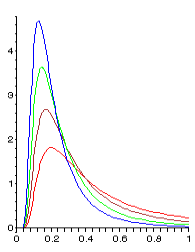
\includegraphics[width=\linewidth, height=4cm, keepaspectratio]{Pictures/distributions/Inverse_chi_squared_pdf.png}
            \caption{Inverse-Chi-square Distribution: PDF}
        \end{figure}
    \end{minipage}
    \hfill
    \begin{minipage}{0.49\linewidth}
        \begin{figure}[H]
            \centering
            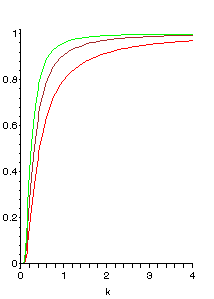
\includegraphics[width=\linewidth, height=4cm, keepaspectratio]{Pictures/distributions/Inverse_chi_squared_cdf.png}
            \caption{Inverse-Chi-square Distribution: CDF}
        \end{figure}
    \end{minipage}
\end{table}

\renewcommand{\arraystretch}{2}
\begin{longtable}{|m{6cm}|p{9cm}|}
    \hline
    \multicolumn{2}{|c|}{\textbf{Inverse-Chi-square Distribution - Info} \cite{wiki/Inverse-chi-squared_distribution}} \\
    \hline\endfirsthead

    \hline
    \multicolumn{2}{|c|}{\textbf{Inverse-Chi-square Distribution - Info - contd.} \cite{wiki/Inverse-chi-squared_distribution}} \\
    \hline\endhead
    
    \hline\endfoot
    \hline\endlastfoot

    \textbf{Statistical parameters} & 
    \\ \hline
    
    \textbf{Support} &
    \\ \hline

    \textbf{Probability Density Function (PDF)} & 
    \\[1ex] \hline
    
    \textbf{Cumulative distribution function (CDF)} & 
    \\ \hline

    \textbf{Mean} & 
    \\[1ex] \hline

    \textbf{Median} & 
    \\[1ex] \hline

    \textbf{Mode} & 
    \\ \hline

    \textbf{Variance} &
    \\[1ex] \hline

    \textbf{Skewness} &
    \\[1ex] \hline

    \textbf{Excess kurtosis} &
    \\[1ex] \hline

    \textbf{Entropy} &
    \\[1ex] \hline

    \textbf{Moment-generating function (MGF)} &
    \\[1ex] \hline

    \textbf{Characteristic function (CF)} &
    \\[1ex] \hline

    \textbf{Probability-generating function (PGF)} &
    \\[1ex] \hline

\end{longtable}
\renewcommand{\arraystretch}{1}












